% Options for packages loaded elsewhere
\PassOptionsToPackage{unicode}{hyperref}
\PassOptionsToPackage{hyphens}{url}
%
\documentclass[
  9pt,
  ignorenonframetext,
  aspectratio=169]{beamer}
\usepackage{pgfpages}
\setbeamertemplate{caption}[numbered]
\setbeamertemplate{caption label separator}{: }
\setbeamercolor{caption name}{fg=normal text.fg}
\beamertemplatenavigationsymbolsempty
% Prevent slide breaks in the middle of a paragraph
\widowpenalties 1 10000
\raggedbottom
\setbeamertemplate{part page}{
  \centering
  \begin{beamercolorbox}[sep=16pt,center]{part title}
    \usebeamerfont{part title}\insertpart\par
  \end{beamercolorbox}
}
\setbeamertemplate{section page}{
  \centering
  \begin{beamercolorbox}[sep=12pt,center]{part title}
    \usebeamerfont{section title}\insertsection\par
  \end{beamercolorbox}
}
\setbeamertemplate{subsection page}{
  \centering
  \begin{beamercolorbox}[sep=8pt,center]{part title}
    \usebeamerfont{subsection title}\insertsubsection\par
  \end{beamercolorbox}
}
\AtBeginPart{
  \frame{\partpage}
}
\AtBeginSection{
  \ifbibliography
  \else
    \frame{\sectionpage}
  \fi
}
\AtBeginSubsection{
  \frame{\subsectionpage}
}
\usepackage{lmodern}
\usepackage{amssymb,amsmath}
\usepackage{ifxetex,ifluatex}
\ifnum 0\ifxetex 1\fi\ifluatex 1\fi=0 % if pdftex
  \usepackage[T1]{fontenc}
  \usepackage[utf8]{inputenc}
  \usepackage{textcomp} % provide euro and other symbols
\else % if luatex or xetex
  \usepackage{unicode-math}
  \defaultfontfeatures{Scale=MatchLowercase}
  \defaultfontfeatures[\rmfamily]{Ligatures=TeX,Scale=1}
\fi
\usetheme[]{Berkeley}
\usecolortheme{dove}
\usefonttheme{structurebold}
% Use upquote if available, for straight quotes in verbatim environments
\IfFileExists{upquote.sty}{\usepackage{upquote}}{}
\IfFileExists{microtype.sty}{% use microtype if available
  \usepackage[]{microtype}
  \UseMicrotypeSet[protrusion]{basicmath} % disable protrusion for tt fonts
}{}
\makeatletter
\@ifundefined{KOMAClassName}{% if non-KOMA class
  \IfFileExists{parskip.sty}{%
    \usepackage{parskip}
  }{% else
    \setlength{\parindent}{0pt}
    \setlength{\parskip}{6pt plus 2pt minus 1pt}}
}{% if KOMA class
  \KOMAoptions{parskip=half}}
\makeatother
\usepackage{xcolor}
\IfFileExists{xurl.sty}{\usepackage{xurl}}{} % add URL line breaks if available
\IfFileExists{bookmark.sty}{\usepackage{bookmark}}{\usepackage{hyperref}}
\hypersetup{
  pdfauthor={Frederico Bertholini},
  hidelinks,
  pdfcreator={LaTeX via pandoc}}
\urlstyle{same} % disable monospaced font for URLs
\newif\ifbibliography
\usepackage{color}
\usepackage{fancyvrb}
\newcommand{\VerbBar}{|}
\newcommand{\VERB}{\Verb[commandchars=\\\{\}]}
\DefineVerbatimEnvironment{Highlighting}{Verbatim}{commandchars=\\\{\}}
% Add ',fontsize=\small' for more characters per line
\usepackage{framed}
\definecolor{shadecolor}{RGB}{248,248,248}
\newenvironment{Shaded}{\begin{snugshade}}{\end{snugshade}}
\newcommand{\AlertTok}[1]{\textcolor[rgb]{0.94,0.16,0.16}{#1}}
\newcommand{\AnnotationTok}[1]{\textcolor[rgb]{0.56,0.35,0.01}{\textbf{\textit{#1}}}}
\newcommand{\AttributeTok}[1]{\textcolor[rgb]{0.77,0.63,0.00}{#1}}
\newcommand{\BaseNTok}[1]{\textcolor[rgb]{0.00,0.00,0.81}{#1}}
\newcommand{\BuiltInTok}[1]{#1}
\newcommand{\CharTok}[1]{\textcolor[rgb]{0.31,0.60,0.02}{#1}}
\newcommand{\CommentTok}[1]{\textcolor[rgb]{0.56,0.35,0.01}{\textit{#1}}}
\newcommand{\CommentVarTok}[1]{\textcolor[rgb]{0.56,0.35,0.01}{\textbf{\textit{#1}}}}
\newcommand{\ConstantTok}[1]{\textcolor[rgb]{0.00,0.00,0.00}{#1}}
\newcommand{\ControlFlowTok}[1]{\textcolor[rgb]{0.13,0.29,0.53}{\textbf{#1}}}
\newcommand{\DataTypeTok}[1]{\textcolor[rgb]{0.13,0.29,0.53}{#1}}
\newcommand{\DecValTok}[1]{\textcolor[rgb]{0.00,0.00,0.81}{#1}}
\newcommand{\DocumentationTok}[1]{\textcolor[rgb]{0.56,0.35,0.01}{\textbf{\textit{#1}}}}
\newcommand{\ErrorTok}[1]{\textcolor[rgb]{0.64,0.00,0.00}{\textbf{#1}}}
\newcommand{\ExtensionTok}[1]{#1}
\newcommand{\FloatTok}[1]{\textcolor[rgb]{0.00,0.00,0.81}{#1}}
\newcommand{\FunctionTok}[1]{\textcolor[rgb]{0.00,0.00,0.00}{#1}}
\newcommand{\ImportTok}[1]{#1}
\newcommand{\InformationTok}[1]{\textcolor[rgb]{0.56,0.35,0.01}{\textbf{\textit{#1}}}}
\newcommand{\KeywordTok}[1]{\textcolor[rgb]{0.13,0.29,0.53}{\textbf{#1}}}
\newcommand{\NormalTok}[1]{#1}
\newcommand{\OperatorTok}[1]{\textcolor[rgb]{0.81,0.36,0.00}{\textbf{#1}}}
\newcommand{\OtherTok}[1]{\textcolor[rgb]{0.56,0.35,0.01}{#1}}
\newcommand{\PreprocessorTok}[1]{\textcolor[rgb]{0.56,0.35,0.01}{\textit{#1}}}
\newcommand{\RegionMarkerTok}[1]{#1}
\newcommand{\SpecialCharTok}[1]{\textcolor[rgb]{0.00,0.00,0.00}{#1}}
\newcommand{\SpecialStringTok}[1]{\textcolor[rgb]{0.31,0.60,0.02}{#1}}
\newcommand{\StringTok}[1]{\textcolor[rgb]{0.31,0.60,0.02}{#1}}
\newcommand{\VariableTok}[1]{\textcolor[rgb]{0.00,0.00,0.00}{#1}}
\newcommand{\VerbatimStringTok}[1]{\textcolor[rgb]{0.31,0.60,0.02}{#1}}
\newcommand{\WarningTok}[1]{\textcolor[rgb]{0.56,0.35,0.01}{\textbf{\textit{#1}}}}
\usepackage{graphicx}
\makeatletter
\def\maxwidth{\ifdim\Gin@nat@width>\linewidth\linewidth\else\Gin@nat@width\fi}
\def\maxheight{\ifdim\Gin@nat@height>\textheight\textheight\else\Gin@nat@height\fi}
\makeatother
% Scale images if necessary, so that they will not overflow the page
% margins by default, and it is still possible to overwrite the defaults
% using explicit options in \includegraphics[width, height, ...]{}
\setkeys{Gin}{width=\maxwidth,height=\maxheight,keepaspectratio}
% Set default figure placement to htbp
\makeatletter
\def\fps@figure{htbp}
\makeatother
\setlength{\emergencystretch}{3em} % prevent overfull lines
\providecommand{\tightlist}{%
  \setlength{\itemsep}{0pt}\setlength{\parskip}{0pt}}
\setcounter{secnumdepth}{5}

\subtitle{Métodos Quantitativos Aplicados à Ciência Política}
\author{Frederico Bertholini}
\date{16.nov.2020}

\begin{document}

\begin{frame}[allowframebreaks]
  \tableofcontents[hideallsubsections]
\end{frame}
\hypertarget{revendo-conteuxfados-da-uxfaltima-aula---rmarkdwon}{%
\section{Revendo conteúdos da última aula -
RMarkdwon}\label{revendo-conteuxfados-da-uxfaltima-aula---rmarkdwon}}

\begin{frame}{.rmd do zero e gh-pages}
\protect\hypertarget{rmd-do-zero-e-gh-pages}{}
\end{frame}

\hypertarget{dados-indicadores-e-escalas}{%
\section{Dados, Indicadores e
escalas}\label{dados-indicadores-e-escalas}}

\begin{frame}[fragile]{Matriz de dados}
\protect\hypertarget{matriz-de-dados}{}
\begin{Shaded}
\begin{Highlighting}[]
\CommentTok{\# Atribuindo o dataframe de exercicio}
\NormalTok{dfe \textless{}{-}}\StringTok{ }\KeywordTok{read\_rds}\NormalTok{(}\StringTok{"dados/dfe.rds"}\NormalTok{)}
\CommentTok{\#}
\end{Highlighting}
\end{Shaded}
\end{frame}

\begin{frame}[fragile]{dataMaid}
\protect\hypertarget{datamaid}{}
\begin{Shaded}
\begin{Highlighting}[]
\CommentTok{\# Codebook dataMaid {-}{-} explicar}
\KeywordTok{attr}\NormalTok{(dfe}\OperatorTok{$}\NormalTok{id, }\StringTok{"label"}\NormalTok{) \textless{}{-}}\StringTok{ "Identificação"}
\KeywordTok{attr}\NormalTok{(dfe}\OperatorTok{$}\NormalTok{id, }\StringTok{"shortDescription"}\NormalTok{) \textless{}{-}}\StringTok{ "Variável de identificação do aluno"}
\KeywordTok{attr}\NormalTok{(dfe}\OperatorTok{$}\NormalTok{media, }\StringTok{"label"}\NormalTok{) \textless{}{-}}\StringTok{ "Média final"}
\KeywordTok{attr}\NormalTok{(dfe}\OperatorTok{$}\NormalTok{media, }\StringTok{"shortDescription"}\NormalTok{) \textless{}{-}}\StringTok{ "Nota do aluno ao final da disciplina"}
\KeywordTok{attr}\NormalTok{(dfe}\OperatorTok{$}\NormalTok{faltas, }\StringTok{"shortDescription"}\NormalTok{) \textless{}{-}}\StringTok{ "Total de faltas ao longo do semestre"}
\KeywordTok{attr}\NormalTok{(dfe}\OperatorTok{$}\NormalTok{turma, }\StringTok{"shortDescription"}\NormalTok{) \textless{}{-}}\StringTok{ "Turma do aluno"}
\KeywordTok{attr}\NormalTok{(dfe}\OperatorTok{$}\NormalTok{idade, }\StringTok{"shortDescription"}\NormalTok{) \textless{}{-}}\StringTok{ "Idade do aluno"}
\KeywordTok{attr}\NormalTok{(dfe}\OperatorTok{$}\NormalTok{interess, }\StringTok{"label"}\NormalTok{) \textless{}{-}}\StringTok{ "Interesse"}
\KeywordTok{attr}\NormalTok{(dfe}\OperatorTok{$}\NormalTok{interess, }\StringTok{"shortDescription"}\NormalTok{) \textless{}{-}}\StringTok{ "Prioridade de interesse do aluno"}
\KeywordTok{attr}\NormalTok{(dfe}\OperatorTok{$}\NormalTok{tempocup, }\StringTok{"shortDescription"}\NormalTok{) \textless{}{-}}\StringTok{ "Tempo de dedicação semanal do aluno"}
\KeywordTok{attr}\NormalTok{(dfe}\OperatorTok{$}\NormalTok{escola, }\StringTok{"shortDescription"}\NormalTok{) \textless{}{-}}\StringTok{ "Tipo de escola onde o aluno cursou ensino médio"}
\KeywordTok{attr}\NormalTok{(dfe}\OperatorTok{$}\NormalTok{estcivil, }\StringTok{"shortDescription"}\NormalTok{) \textless{}{-}}\StringTok{ "Estado civil do aluno"}

\CommentTok{\# makeCodebook(dfe,file = "cb\_dfe.rmd")}
\end{Highlighting}
\end{Shaded}

\href{http://biostat.mc.vanderbilt.edu/wiki/pub/Main/MollyOlson/R-ladies-datamaid.html}{R
Ladies - dataMaid}
\end{frame}

\begin{frame}{Índices e escalas}
\protect\hypertarget{uxedndices-e-escalas}{}
Ordinais

\begin{itemize}
\tightlist
\item
  Escala
\end{itemize}

-- Atribuições ao padrão de resposta

-- Pode conter vários itens

\begin{itemize}
\tightlist
\item
  Índice
\end{itemize}

-- Compostos por itens (multidimensional)

-- cada item é uma variável
\end{frame}

\begin{frame}{Critérios}
\protect\hypertarget{crituxe9rios}{}
\begin{itemize}
\item
  Validade (interna e externa)
\item
  Variância
\item
  Correlação (bivariada e multivariada)
\item
  Outras propriedades consagradas (Januzzi)
\end{itemize}
\end{frame}

\begin{frame}{}
\protect\hypertarget{section}{}
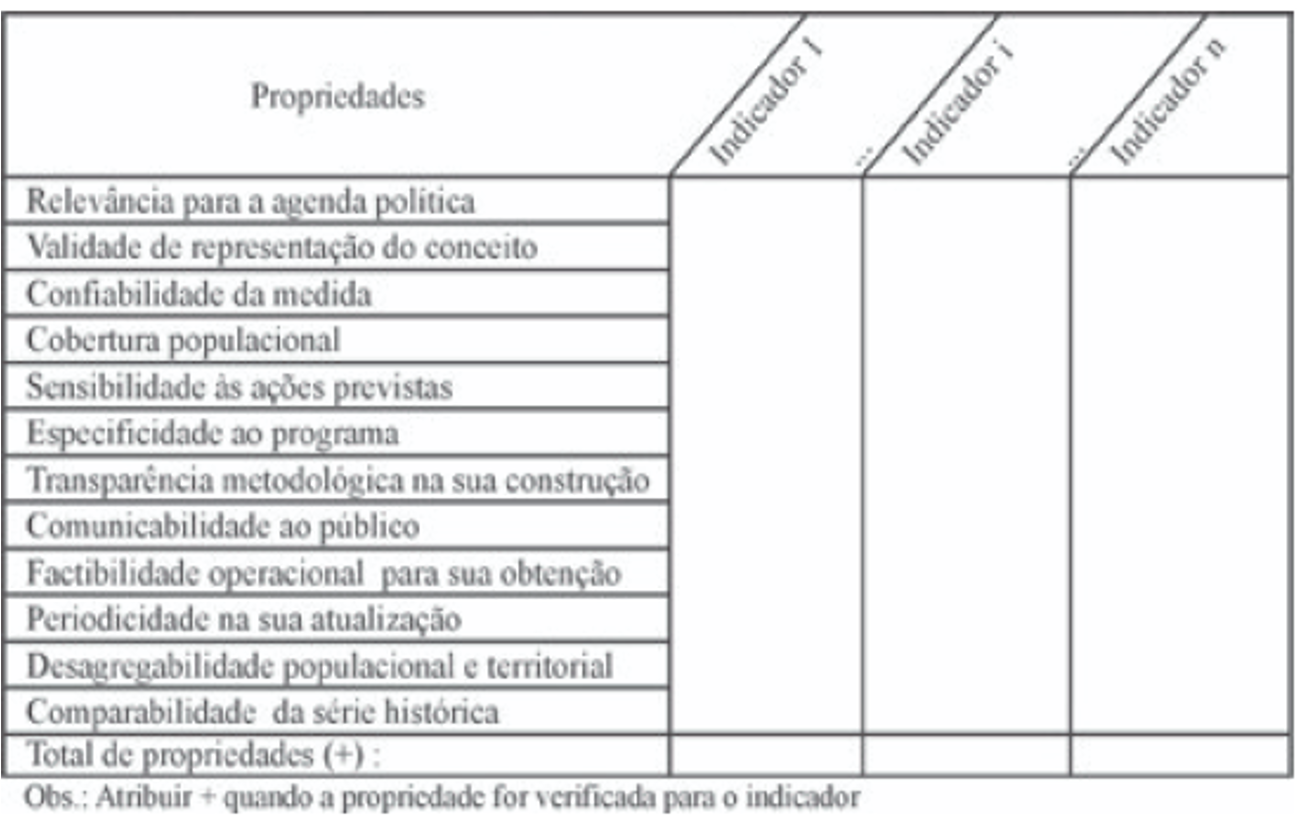
\includegraphics{imgs/indicadores}
\end{frame}

\begin{frame}{tribuição de pontos}
\protect\hypertarget{tribuiuxe7uxe3o-de-pontos}{}
Escalas de respostas

\begin{itemize}
\item
  amplitude
\item
  Não resposta
\item
  pesos
\end{itemize}
\end{frame}

\begin{frame}{Tipos}
\protect\hypertarget{tipos}{}
\begin{itemize}
\item
  Likert
\item
  Feeling thermometer
\end{itemize}

Menos conhecidas (e utilizadas)

\begin{itemize}
\item
  Bogartus (distância social)
\item
  Thurstone
\item
  Guttman
\end{itemize}

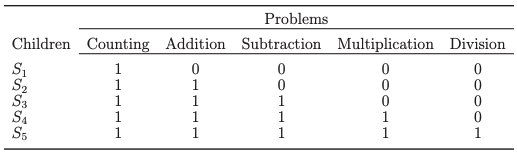
\includegraphics{imgs/guttman}
\end{frame}

\begin{frame}{Testes de confiabilidade - Cronbach}
\protect\hypertarget{testes-de-confiabilidade---cronbach}{}
Exemplo Cervi

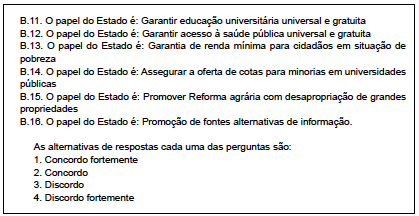
\includegraphics{imgs/excervi1.png}
\end{frame}

\begin{frame}{}
\protect\hypertarget{section-1}{}
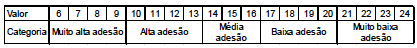
\includegraphics{imgs/excervi2.png}
\end{frame}

\begin{frame}{}
\protect\hypertarget{section-2}{}
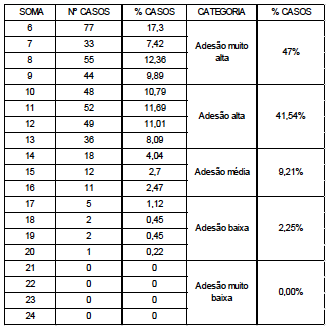
\includegraphics{imgs/result_dados.png}
\end{frame}

\begin{frame}{Princípios}
\protect\hypertarget{princuxedpios}{}
\begin{itemize}
\item
  Criterion-related
\item
  Content
\item
  Construct
\end{itemize}

Lógica:

\[x = t + e \]

Onde:

\(x\) é a medida empírica a ser estudada

\(t\) é a parte explicada da variação

\(e\) é o erro randômico (aleatório)

Vamos olhar isso melhor em inferência.
\end{frame}

\begin{frame}{Fórmula}
\protect\hypertarget{fuxf3rmula}{}
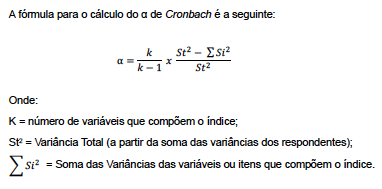
\includegraphics{imgs/formula_crb.png}
\end{frame}

\begin{frame}[fragile]{Cronbach}
\protect\hypertarget{cronbach}{}
Usando o pacote psych

\begin{Shaded}
\begin{Highlighting}[]
\NormalTok{r4 \textless{}{-}}\StringTok{ }\NormalTok{psych}\OperatorTok{::}\KeywordTok{sim.congeneric}\NormalTok{()}
\NormalTok{crb \textless{}{-}}\StringTok{ }\NormalTok{psych}\OperatorTok{::}\KeywordTok{alpha}\NormalTok{(r4)}
\KeywordTok{summary}\NormalTok{(crb)}
\end{Highlighting}
\end{Shaded}

\begin{verbatim}
Reliability analysis   
 raw_alpha std.alpha G6(smc) average_r S/N median_r
      0.74      0.74    0.69      0.42 2.9     0.41
\end{verbatim}
\end{frame}

\begin{frame}{}
\protect\hypertarget{section-3}{}
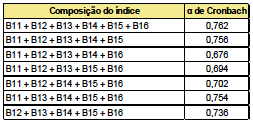
\includegraphics{imgs/result_exemplo.png}
\end{frame}

\begin{frame}{Mais info}
\protect\hypertarget{mais-info}{}
\href{http://personality-project.org/r/psych/}{Pacote psych}

\href{https://www.r-bloggers.com/2016/08/five-ways-to-calculate-internal-consistency/}{Consistência
Interna}
\end{frame}

\begin{frame}{Indicadores estatísticos}
\protect\hypertarget{indicadores-estatuxedsticos}{}
Razão: \(Z=X/Y\)

Proporção: \(Z=X/(Y+X)\)

Percentagem: \(Proporção*100\)

Taxa: \(eventos/exposição ao risco\)
\end{frame}

\hypertarget{indicadores-parlamentares-e-eleitorais}{%
\section{Indicadores parlamentares e
eleitorais}\label{indicadores-parlamentares-e-eleitorais}}

\begin{frame}{Parlamentares - Índice de fracionalização}
\protect\hypertarget{parlamentares---uxedndice-de-fracionalizauxe7uxe3o}{}
\end{frame}

\begin{frame}{Parlamentares - Índice de fracionalização máxima}
\protect\hypertarget{parlamentares---uxedndice-de-fracionalizauxe7uxe3o-muxe1xima}{}
\end{frame}

\begin{frame}{Parlamentares - Índice de fragmentação}
\protect\hypertarget{parlamentares---uxedndice-de-fragmentauxe7uxe3o}{}
\end{frame}

\begin{frame}{Parlamentares - Número efetivo de partidos}
\protect\hypertarget{parlamentares---nuxfamero-efetivo-de-partidos}{}
\[ \Huge \frac{1}{\sum pe^{2}} \]
\end{frame}

\begin{frame}{Parlamentares - Renovação}
\protect\hypertarget{parlamentares---renovauxe7uxe3o}{}
\begingroup\Large

\begin{equation*}
Y_{ij} = [\beta_0 + \beta_1 (\text{Dose}-300)] + [\varepsilon_{ij}]
\end{equation*} \endgroup
\end{frame}

\begin{frame}{Eleitorais}
\protect\hypertarget{eleitorais}{}
\end{frame}

\begin{frame}{Mais recursos}
\protect\hypertarget{mais-recursos}{}
\href{https://github.com/rOpenGov/psData}{psData}

\href{http://ropengov.github.io/projects/}{rOpenGov}

\href{http://ropengov.github.io/rqog/}{QoG}

\href{https://cran.r-project.org/web/packages/electoral/index.html}{electoral}
\end{frame}

\begin{frame}[fragile]{Representações descritivas de dados - Tabela}
\protect\hypertarget{representauxe7uxf5es-descritivas-de-dados---tabela}{}
\begin{Shaded}
\begin{Highlighting}[]
\CommentTok{\# Com tabyl}
\NormalTok{dfe }\OperatorTok{\%\textgreater{}\%}
\StringTok{  }\KeywordTok{drop\_na}\NormalTok{(interess,estcivil) }\OperatorTok{\%\textgreater{}\%}\StringTok{ }\CommentTok{\# retirando NAs}
\StringTok{  }\NormalTok{janitor}\OperatorTok{::}\KeywordTok{tabyl}\NormalTok{(interess,estcivil) }\OperatorTok{\%\textgreater{}\%}\StringTok{ }\CommentTok{\# tabela cruzada}
\StringTok{  }\NormalTok{janitor}\OperatorTok{::}\KeywordTok{adorn\_percentages}\NormalTok{(}\StringTok{"col"}\NormalTok{) }\OperatorTok{\%\textgreater{}\%}
\StringTok{  }\NormalTok{janitor}\OperatorTok{::}\KeywordTok{adorn\_pct\_formatting}\NormalTok{()}
\end{Highlighting}
\end{Shaded}

\begin{verbatim}
   interess Casado Solteiro
 Secundário  29.4%    45.0%
  Principal  70.6%    55.0%
\end{verbatim}
\end{frame}

\begin{frame}[fragile]{Representações descritivas de dados - Histograma}
\protect\hypertarget{representauxe7uxf5es-descritivas-de-dados---histograma}{}
\begin{Shaded}
\begin{Highlighting}[]
\NormalTok{dfe }\OperatorTok{\%\textgreater{}\%}
\StringTok{  }\KeywordTok{ggplot}\NormalTok{() }\OperatorTok{+}
\StringTok{  }\KeywordTok{geom\_histogram}\NormalTok{(}\KeywordTok{aes}\NormalTok{(media),}\DataTypeTok{bins=}\DecValTok{4}\NormalTok{)}
\end{Highlighting}
\end{Shaded}

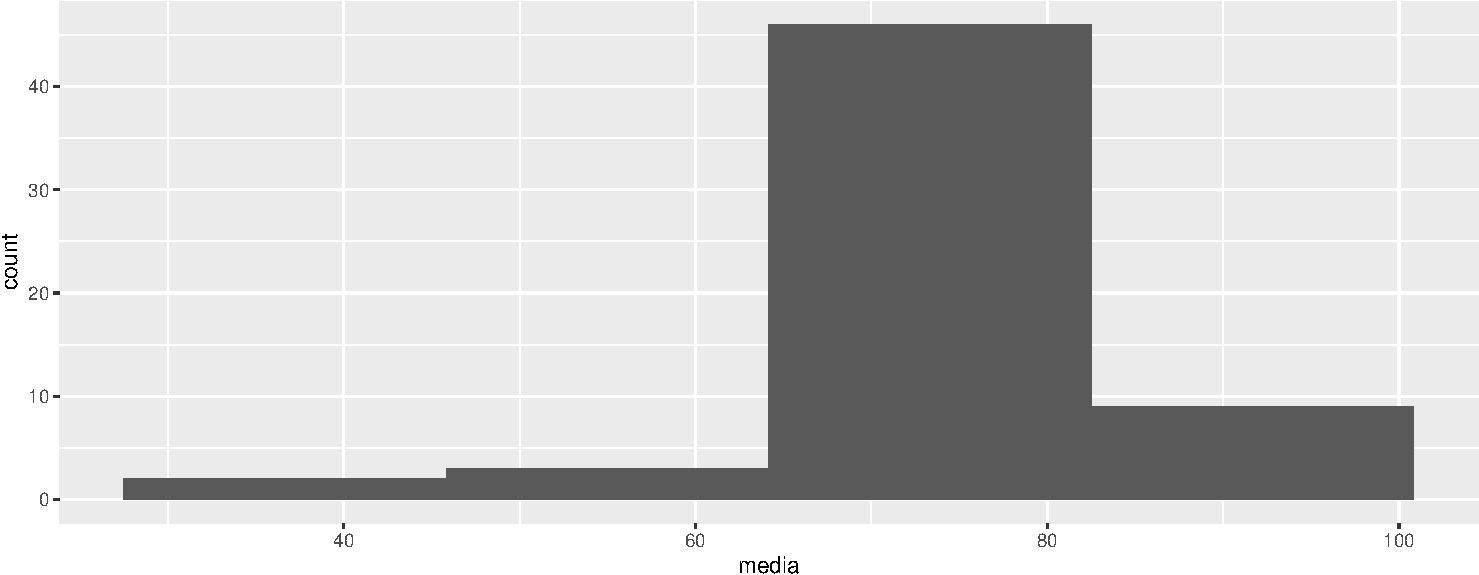
\includegraphics{aula_08_files/figure-beamer/unnamed-chunk-5-1.pdf}
\end{frame}

\begin{frame}[fragile]{Representações descritivas de dados - Gráfico de
dispersão}
\protect\hypertarget{representauxe7uxf5es-descritivas-de-dados---gruxe1fico-de-dispersuxe3o}{}
\begin{Shaded}
\begin{Highlighting}[]
\NormalTok{dfe }\OperatorTok{\%\textgreater{}\%}
\StringTok{  }\KeywordTok{ggplot}\NormalTok{(}\KeywordTok{aes}\NormalTok{(}\DataTypeTok{y=}\NormalTok{media,}\DataTypeTok{x=}\NormalTok{idade,}\DataTypeTok{group=}\NormalTok{escola)) }\OperatorTok{+}
\StringTok{  }\KeywordTok{geom\_point}\NormalTok{() }\OperatorTok{+}
\StringTok{  }\KeywordTok{geom\_smooth}\NormalTok{(}\DataTypeTok{method=}\StringTok{"lm"}\NormalTok{)}
\end{Highlighting}
\end{Shaded}

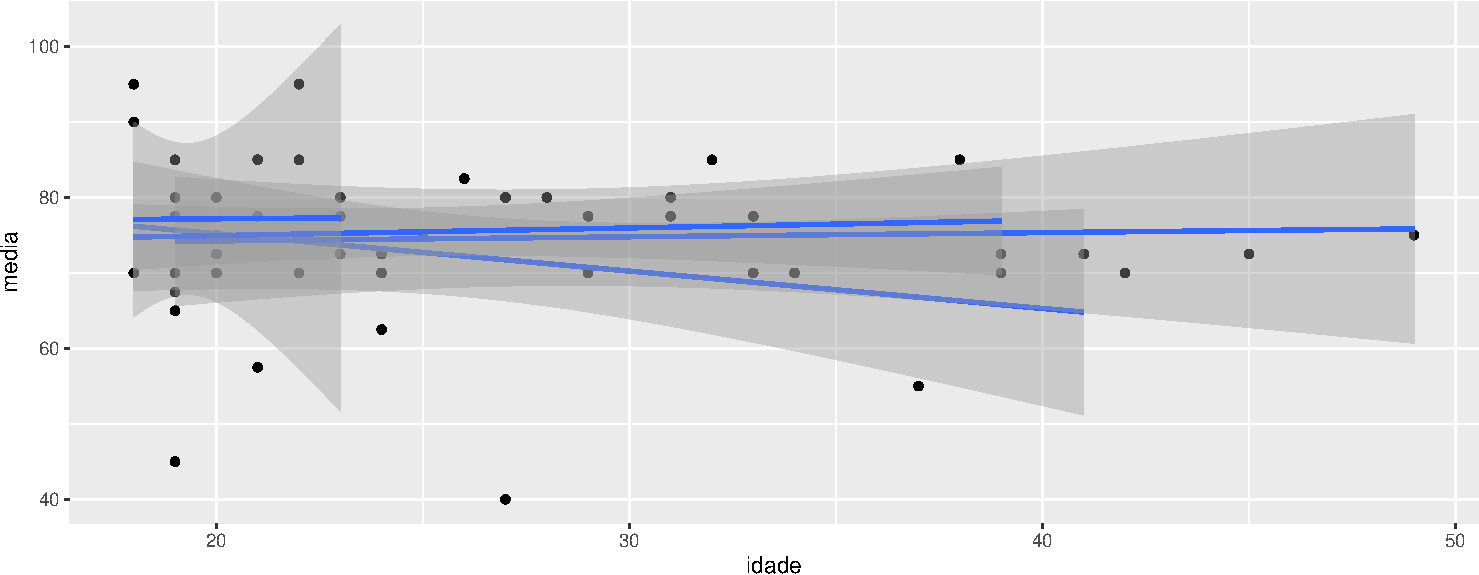
\includegraphics{aula_08_files/figure-beamer/unnamed-chunk-6-1.pdf}
\end{frame}

\begin{frame}[fragile]{Representações descritivas de dados - Binário}
\protect\hypertarget{representauxe7uxf5es-descritivas-de-dados---binuxe1rio}{}
\begin{Shaded}
\begin{Highlighting}[]
\NormalTok{dfe }\OperatorTok{\%\textgreater{}\%}
\StringTok{  }\KeywordTok{drop\_na}\NormalTok{() }\OperatorTok{\%\textgreater{}\%}
\StringTok{  }\KeywordTok{ggplot}\NormalTok{() }\OperatorTok{+}
\StringTok{  }\KeywordTok{geom\_bar}\NormalTok{(}\KeywordTok{aes}\NormalTok{(}\DataTypeTok{fill=}\NormalTok{estcivil,}\DataTypeTok{y=}\NormalTok{estcivil),}\DataTypeTok{position =} \KeywordTok{position\_stack}\NormalTok{(}\DataTypeTok{reverse =} \OtherTok{TRUE}\NormalTok{),}\DataTypeTok{stat =} \StringTok{"count"}\NormalTok{)}
\end{Highlighting}
\end{Shaded}

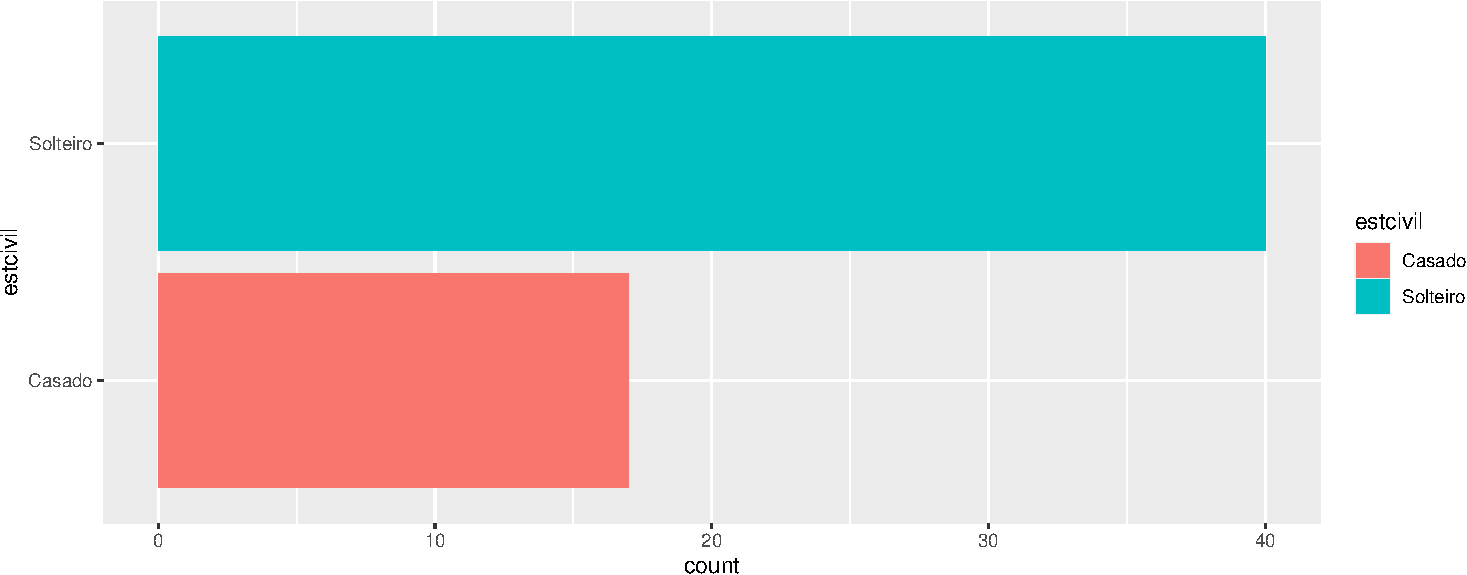
\includegraphics{aula_08_files/figure-beamer/unnamed-chunk-7-1.pdf}
\end{frame}

\begin{frame}[fragile]{Representações descritivas de dados - Box plot}
\protect\hypertarget{representauxe7uxf5es-descritivas-de-dados---box-plot}{}
\begin{Shaded}
\begin{Highlighting}[]
\NormalTok{dfe }\OperatorTok{\%\textgreater{}\%}
\StringTok{  }\KeywordTok{drop\_na}\NormalTok{() }\OperatorTok{\%\textgreater{}\%}
\StringTok{  }\NormalTok{ggpubr}\OperatorTok{::}\KeywordTok{ggboxplot}\NormalTok{(}\DataTypeTok{x=}\StringTok{"estcivil"}\NormalTok{,}\DataTypeTok{y=}\StringTok{"idade"}\NormalTok{,}\DataTypeTok{fill =} \StringTok{"estcivil"}\NormalTok{)}
\end{Highlighting}
\end{Shaded}

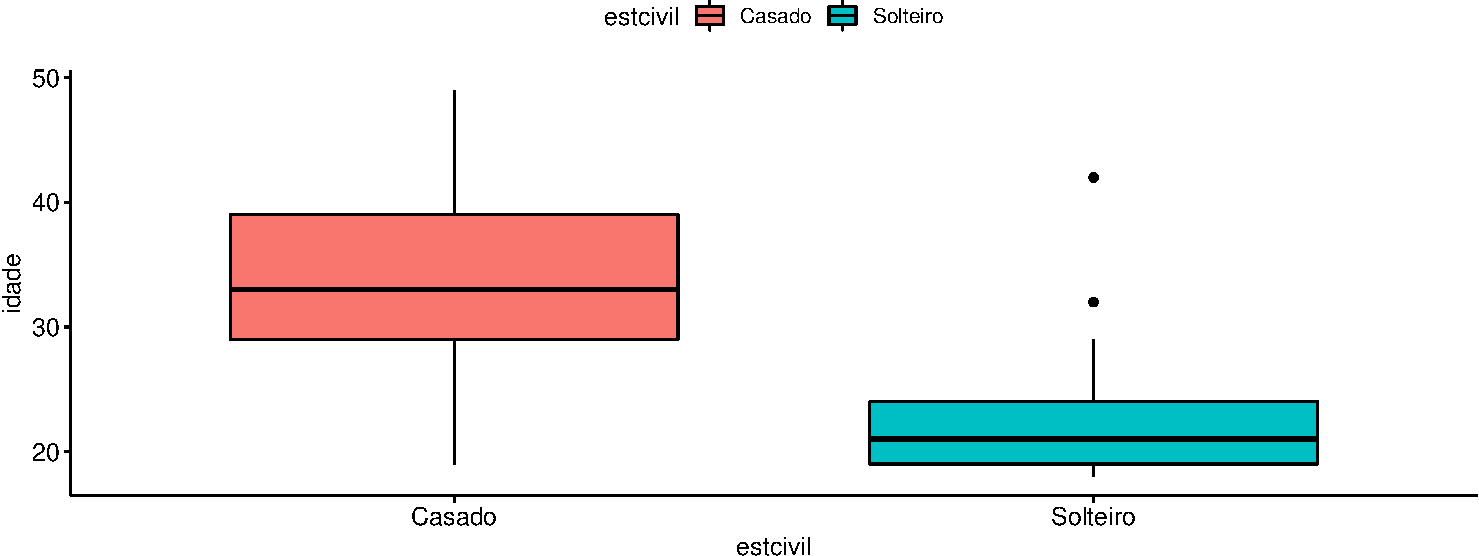
\includegraphics{aula_08_files/figure-beamer/unnamed-chunk-8-1.pdf}
\end{frame}

\hypertarget{medidas-de-posiuxe7uxe3o}{%
\section{Medidas de posição}\label{medidas-de-posiuxe7uxe3o}}

\begin{frame}{Medidas de posição}
\protect\hypertarget{medidas-de-posiuxe7uxe3o-1}{}
As medidas de posição trazem informação sobre a localização dos dados no
seu conjunto de possíveis valores.
\end{frame}

\begin{frame}[fragile]{Média aritmética}
\protect\hypertarget{muxe9dia-aritmuxe9tica}{}
A média aritmética é definida pela soma das observações dividida pelo
número total de observações.

Exemplo: sejam \(x_1, ..., x_n\) \(n\) observações de uma variável \(X\)
qualquer. A média é dada pela expressão

\(\frac{\sum_{i=1}^{n}x_i}{n} = \frac{x_1 + x_2 + ... + x_n}{n}\)

No R:

\begin{Shaded}
\begin{Highlighting}[]
\NormalTok{dfe }\OperatorTok{\%\textgreater{}\%}
\StringTok{  }\KeywordTok{pull}\NormalTok{(media) }\OperatorTok{\%\textgreater{}\%}
\StringTok{  }\KeywordTok{mean}\NormalTok{(}\DataTypeTok{na.rm=}\NormalTok{T)}
\end{Highlighting}
\end{Shaded}

\begin{verbatim}
[1] 74.375
\end{verbatim}
\end{frame}

\begin{frame}{Média ponderada}
\protect\hypertarget{muxe9dia-ponderada}{}
\end{frame}

\begin{frame}{Mediana}
\protect\hypertarget{mediana}{}
A mediana é a observação que ocupa a posição central dos dados.

Exemplo 1 (número ímpar de observações): vamos considerar o seguinte
conjunto de observações: 3, 7, 10, 5, 2, 1, 1.

Para calcular a mediana, primeiramente ordenamos os dados: 1, 1, 2, 3,
5, 7, 10.

É fácil verificar que a observação que ocupa a posição central é o valor
3. Portanto, 3 é a mediana desse conjunto de valores.

Exemplo 2 (número par de observações): vamos considerar agora o seguinte
conjunto de observações: 15, 3, 2, 0, 9, 17.

Ordenanando os dados, temos: 0, 2, 3, 9, 15, 17.

Neste caso, a mediana será dada pela média entre as duas observações
centrais, isto é, \((3 + 9)/2 = 6\).
\end{frame}

\begin{frame}{Moda}
\protect\hypertarget{moda}{}
A moda é a observação mais frequente do conjunto de valores observados.

Exemplo: no conjunto de observações \{3, 5, 10, 11, 11, 20\}, a
observação 11 aparece 2 vezes enquanto as demais apenas 1 vez. Portanto,
11 é a moda desse conjunto.
\end{frame}

\hypertarget{medidas-de-dispersuxe3o}{%
\section{Medidas de dispersão}\label{medidas-de-dispersuxe3o}}

\begin{frame}{Medidas de dispersão}
\protect\hypertarget{medidas-de-dispersuxe3o-1}{}
O resumo de um conjunto de dados por uma única medida de posição central
não traz informação sobre a variabilidade das observações.

Um critério frequentemente usado para avaliar a dispersão de um conjunto
de observações é aquele que mede a dispersão dos dados em torno da sua
média.
\end{frame}

\begin{frame}{Amplitude e Quantis}
\protect\hypertarget{amplitude-e-quantis}{}
Amplitude = valor máximo - valor mínimo

A mediana é uma medida que deixa metade dos dados abaixo dela e metade
acima. De modo geral, podemos definir a medida \(q_p\), \(0 < p < 100\),
tal que \(p%
\) das observações sejam menores que \(q_p\). Esta medida é chamada de
quantil de ordem \(p\).

Alguns quantis são bastante utilizados na prática. São eles

\(Q1 = q_{25\%}\) (primeiro quartil)

\(Q2 = q_{50\%}\) (mediana)

\(Q3 = q_{75\%}\) (terceiro quartil)

Observe que os \(q_{0\%}\) e \(q_{100\%}\) denotam, respectivamente, o
mínimo e o máximo de conjunto de dados.
\end{frame}

\begin{frame}{Variância}
\protect\hypertarget{variuxe2ncia}{}
Sejam \(x_1, x_2, ..., x_n\) \(n\) observações de uma variável
quantitativa \(X\). Seja \(\bar{x}\) a média dessas observações.

Vamos observar, então, os desvios das observações em relação à média
\(\bar{x}\), isto é, \(x_i - \bar{x}\), para \(i = 1, ..., n\).

\textbf{Ideia 1}: usar como medida de dispersão a soma desses desvios,
isto é,

\[ \Large
\sum_{i=1}^{n}(x_i - \bar{x}).
\]
\end{frame}

\begin{frame}{}
\protect\hypertarget{section-4}{}
\textbf{Problema 1}: para qualquer conjunto de observações

\[ \Large
\sum_{i=1}^{n}(x_i - \bar{x}) = 0.
\]

\textbf{Ideia 2}: considerar a soma do quadrado dos desvios, dada por

\[ \Large
\sum_{i=1}^{n}(x_i - \bar{x})^2
\]
\end{frame}

\begin{frame}{}
\protect\hypertarget{section-5}{}
\textbf{Problema 2}: não podemos comparar conjuntos de observações de
tamanhos diferentes.

\textbf{Ideia 3}: utilizar a média desses desvios quadráticos.

Sendo assim, definimos a medida de dispersão conhecida como
\textbf{variância} da seguinte forma:

\[ \Large
var(X) = \frac{\sum_{i=1}^{n}(x_i - \bar{x})^2}{n}
\]
\end{frame}

\begin{frame}{Desvio padrão}
\protect\hypertarget{desvio-padruxe3o}{}
A utilização da variância como medida de dispersão pode ainda causar um
problema de interpretação, pois a sua dimensão é igual ao quadrado da
dimensão dos dados. Sendo assim, costuma-se usar o desvio padrão,
definido por

\[ \Large
dp(X) = \sqrt{var(X)} = \sqrt{\frac{\sum_{i=1}^{n}(x_i - \bar{x})^2}{n}}
\]
\end{frame}

\begin{frame}{Coeficiente de variação}
\protect\hypertarget{coeficiente-de-variauxe7uxe3o}{}
Medida relativa -\textgreater{} que proporção da média é o desvio-padrão

\[ \Huge 
\frac{dp}{média}
\]
\end{frame}

\begin{frame}[fragile]{vendo média, mediana e distribuições}
\protect\hypertarget{vendo-muxe9dia-mediana-e-distribuiuxe7uxf5es}{}
\begin{Shaded}
\begin{Highlighting}[]
\NormalTok{dfe }\OperatorTok{\%\textgreater{}\%}\StringTok{ }\KeywordTok{ggplot}\NormalTok{() }\OperatorTok{+}
\StringTok{  }\KeywordTok{geom\_density}\NormalTok{(}\KeywordTok{aes}\NormalTok{(}\DataTypeTok{x=}\NormalTok{media),}\DataTypeTok{alpha=}\NormalTok{.}\DecValTok{5}\NormalTok{,}\DataTypeTok{color=}\OtherTok{NA}\NormalTok{) }\OperatorTok{+}
\StringTok{  }\KeywordTok{geom\_vline}\NormalTok{(}\DataTypeTok{data=}\NormalTok{ . }\OperatorTok{\%\textgreater{}\%}\StringTok{ }\CommentTok{\#group\_by(1) \%\textgreater{}\%}
\StringTok{               }\KeywordTok{summarise}\NormalTok{(}\DataTypeTok{media\_=}\KeywordTok{mean}\NormalTok{(media,}\DataTypeTok{na.rm=}\NormalTok{T),}\DataTypeTok{mediana=}\KeywordTok{median}\NormalTok{(media,}\DataTypeTok{na.rm =}\NormalTok{ T)) }\OperatorTok{\%\textgreater{}\%}
\StringTok{               }\KeywordTok{pivot\_longer}\NormalTok{(media\_}\OperatorTok{:}\NormalTok{mediana),}
             \KeywordTok{aes}\NormalTok{(}\DataTypeTok{xintercept=}\NormalTok{value,}\DataTypeTok{linetype=}\NormalTok{name))}
\end{Highlighting}
\end{Shaded}

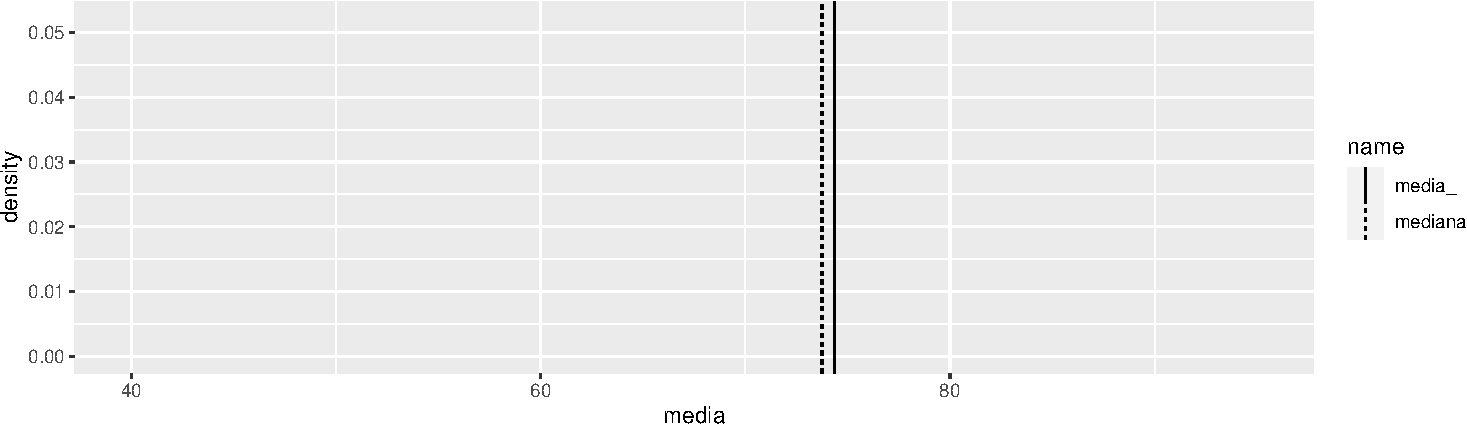
\includegraphics{aula_08_files/figure-beamer/unnamed-chunk-10-1.pdf}
\end{frame}

\begin{frame}[fragile]{vendo média, mediana e distribuições}
\protect\hypertarget{vendo-muxe9dia-mediana-e-distribuiuxe7uxf5es-1}{}
\begin{Shaded}
\begin{Highlighting}[]
\NormalTok{dfe }\OperatorTok{\%\textgreater{}\%}\StringTok{ }\KeywordTok{ggplot}\NormalTok{() }\OperatorTok{+}
\StringTok{  }\KeywordTok{geom\_density}\NormalTok{(}\KeywordTok{aes}\NormalTok{(}\DataTypeTok{fill=}\NormalTok{turma,}\DataTypeTok{x=}\NormalTok{media),}\DataTypeTok{alpha=}\NormalTok{.}\DecValTok{5}\NormalTok{,}\DataTypeTok{color=}\OtherTok{NA}\NormalTok{) }\OperatorTok{+}
\StringTok{  }\KeywordTok{geom\_vline}\NormalTok{(}\DataTypeTok{data=}\NormalTok{ . }\OperatorTok{\%\textgreater{}\%}\StringTok{ }\KeywordTok{group\_by}\NormalTok{(turma) }\OperatorTok{\%\textgreater{}\%}
\StringTok{               }\KeywordTok{summarise}\NormalTok{(}\DataTypeTok{media\_=}\KeywordTok{mean}\NormalTok{(media,}\DataTypeTok{na.rm=}\NormalTok{T),}\DataTypeTok{mediana=}\KeywordTok{median}\NormalTok{(media,}\DataTypeTok{na.rm =}\NormalTok{ T)) }\OperatorTok{\%\textgreater{}\%}\StringTok{ }
\StringTok{               }\NormalTok{dplyr}\OperatorTok{::}\KeywordTok{rename}\NormalTok{(}\DataTypeTok{media=}\NormalTok{media\_) }\OperatorTok{\%\textgreater{}\%}\StringTok{ }\KeywordTok{pivot\_longer}\NormalTok{(media}\OperatorTok{:}\NormalTok{mediana) ,}
             \KeywordTok{aes}\NormalTok{(}\DataTypeTok{color=}\NormalTok{turma,}\DataTypeTok{xintercept=}\NormalTok{value,}\DataTypeTok{linetype=}\NormalTok{name))}
\end{Highlighting}
\end{Shaded}

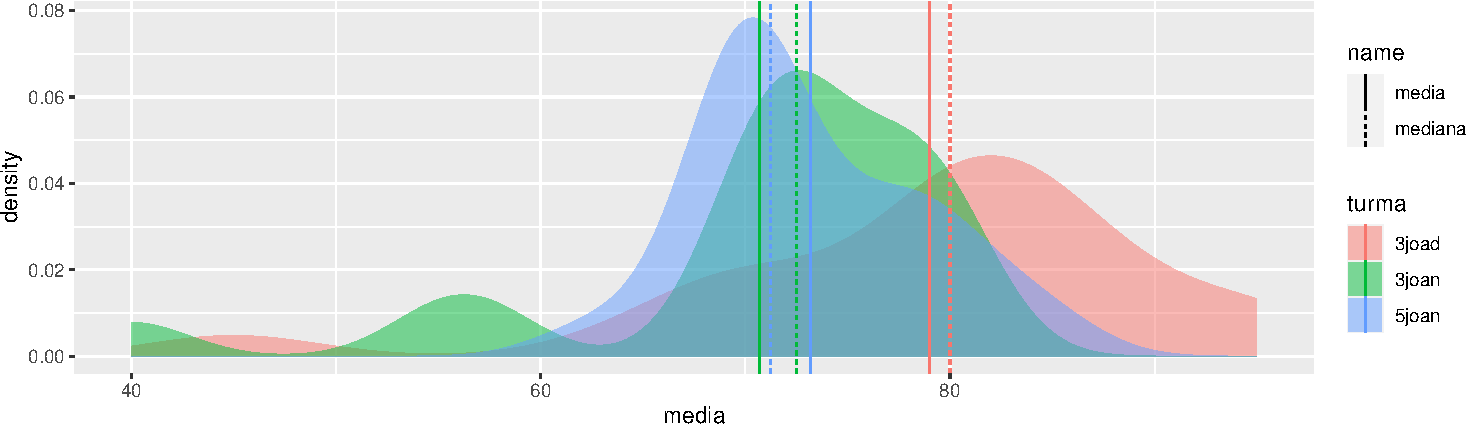
\includegraphics{aula_08_files/figure-beamer/unnamed-chunk-11-1.pdf}
\end{frame}

\begin{frame}{Medidas de assimetria e curtose}
\protect\hypertarget{medidas-de-assimetria-e-curtose}{}
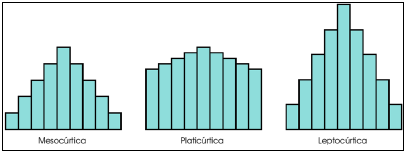
\includegraphics{imgs/curtose.png}

Coeficiente de Assimteria de Pearson = \(média - moda\)

Assimetria adimensional = \(\frac{média - moda}{dp}\)

Coeficiente quartílico de assimetria = \(3*\frac{média-mediana}{dp}\)
\end{frame}

\hypertarget{surveys-e-planejamento}{%
\section{Surveys e planejamento}\label{surveys-e-planejamento}}

\end{document}
